\documentclass{article}

\usepackage[english]{babel}
\usepackage{csquotes}

\usepackage{amsmath}
\usepackage{amssymb}

\usepackage{booktabs}

\usepackage[
    backend=biber,
    style=ieee,
    maxnames=99,
]{biblatex}
\addbibresource{references.bib}
\usepackage{hyperref}
\hypersetup{hidelinks}
% fix capitalization of section, subsection
\addto\extrasenglish{\def\sectionautorefname{Section}}
\addto\extrasenglish{\def\subsectionautorefname{Subsection}}

\usepackage{tikz}
\usetikzlibrary{
  automata,
  positioning,
  arrows, arrows.meta,
  calc, backgrounds, quotes,
  patterns, fit
}
\tikzset{
  op/.style={
    font=\footnotesize,
    state,
    minimum size=56.0pt,
    fill=white,
    scale=0.9,
  },
  head/.style={
    op,
    accepting,
  },
  edge/.style={
    ->,
    >={Stealth[round]},
  },
  pred/.style={
    edge,
  },
  anchorref/.style={
    edge,
    blue,
    densely dashed,
  },
  stepmarker/.style={
    font=\footnotesize,
    fill=black!10,
  },
  stepline/.style={
    edge,
    black!70,
    dotted,
    semithick,
    -,
  },
}

% verbatim does not work here, use some alternative like listing or minted?
\newenvironment{codeblock}{
    \begin{small}
    \begin{verbatim}
}{
    \end{verbatim}
    \end{small}
}
\newcommand{\code}[1]{\texttt{#1}}
\newcommand{\setop}[5][set]{$\mathit{#1}_{#2}^{#3}(#4, #5)$}
\newcommand{\var}[1]{\mathit{#1}}
\newcommand{\deltaI}[1]{\(\delta I_{\text{#1}}\)}
\newcommand{\deltaO}[1][]{\(\delta O_{\text{#1}}\)}

\begin{document}

\title{Research Proposal: Expressing CRDTs with Datalog}
\author{Leo Stewen}

\maketitle

Today's CRDT implementations are built around the in-memory,
object-oriented paradigm~\cite{laddad2022keep} in which there is an API
in the application language with some predefined interface that
specifies how to update and read the state of a CRDT.
However, there is also the idea of defining data structures like CRDTs
as relational queries~\cite{kleppmann2018data}.
In this alternative model, the state of a CRDT is obtained through a query over
relations of operations that are gossiped across replicas.
This research aims to explore this alternative model further and
to utilize Datalog as a potential query language due to its elegance in
expressing recursive queries, which we believe to be a fundamental aspect in
defining CRDTs as queries.
Furthermore, the declarative nature of a query language may be easier to work
with than lower-level, in-memory, object-oriented data structures.

\section{Background on CRDTs and Coordination-free Environments}

Convergent Replicated Data Types (CRDTs)\footnote{
	Although CRDTs are often referred to as \emph{Conflict-free} Replicated
	Data Types, we use the term \emph{convergent} here because the former term
	is a bit misleading as conflicts can still occur
	(see \autoref{sec:motivating_example}).
	We think CRDTs are better characterized by their property that diverging
	replicas eventually \emph{converge} to the same state,
	given the delivery of the same updates,
	and that state may include conflicts, e.g., within a register.
} try to solve the problems arising from asynchronous collaboration over
message-passing (packet-switched) networks on the data structure level.
In these coordination-free environments, in which replicas can be offline
for extended periods of time but are still permitted to write (and read)
to (from) their local state,
the naive delivery of messages allows messages to be arbitrarily delayed,
to be reordered, and the same message may be delivered multiple times.
CRDTs account for these challenges by augmenting messages (hereafter updates
to the CRDT) with additional metadata (1) to preserve the user's intention
in the ``best'' possible manner and (2) to ensure the convergence of replicas,
even after temporary divergence.
This model is great for two things: excellent availability and latency for writes.
Reads also offer excellent latency but may be stale insofar that they do not
reflect the full global state.
As a consequence of allowing offline writes,
application specific invariants (beyond the ones guaranteed by the concrete CRDT)
may be violated on the aggregate level after convergence,
even though each write individually respected the invariants (based on their
respective replica's state at write creation time).
However, this issue sometimes even affects the ``guarantees'' of a CRDT:
Their correct definition is complex and error-prone,
let alone proving their convergence, even for people familiar with distributed
systems~\cite{kleppmann2022assessing, gomes2017verifying}.
Hence, we want to explore a system based on queries over relational data
which trivially fulfills the convergence property of CRDTs.
This allows application developers without a background in eventual
consistency to formulate their own, application-specific CRDTs without
having to worry about convergence.

\section{A Primer on Datalog}
\label{sec:primer_datalog}

Datalog~\cite{green2013datalog} is a declarative logic programming language
that can be used to express queries over a database.
A Datalog program (query) consists of a set of rules,
which are used to derive new facts from existing ones.
The rules are written in the form of Horn clauses
which are logical implications of the form

\[
	\underbrace{
	\underbrace{A}_{\text{head}}
	\text{ :- }
	\underbrace{
	\underbrace{B_1}_{\text{atom}},
	\underbrace{B_2}_{\text{atom}},
	\ldots,
	\underbrace{B_n}_{\text{atom}}
	}_{\text{body}}
	}_{\text{rule}}
\]

\noindent{}and can be read (rather from right to left) as
``$B_1$ and $B_2$ and \ldots\ and $B_n$ imply $A$''.
Written in more mathematical notation, this can be expressed as:

\[
	\begin{aligned}
		                & A \Leftarrow B_1 \land B_2 \land \ldots \land B_n          \\
		\Leftrightarrow & A \lor \lnot B_1 \lor \lnot B_2 \lor \ldots \lor \lnot B_n
	\end{aligned}
\]

If there are multiple rules with the same head,
the bodies are connected with a disjunction~\cite{abo2024convergence}.
Special cases of Horn clauses are facts (fact rules, base atoms),
which are rules without a body, that is $n=0$, e.g., \( A \text{ :- } \text{true} \),
and they are assumed to be unconditionally true.
These facts or \emph{base atoms} are the basis of a Datalog query and
define \emph{extensional database predicates} (EDB)
from which \emph{derived atoms} are created,
which then form \emph{intensional database predicates} (IDB).

%Terminology:

%\begin{itemize}
%	\item \textbf{Rule:} A Horn clause.
%	\item \textbf{Head:} The predicate that is derived by the rule.
%	\item \textbf{Body:} The predicates that need to be true in order to derive the head.
%	\item \textbf{Term:} A constant or a variable.
%	\item \textbf{Atom:} A function (also: predicate symbol) with a list of terms as arguments.
%	      The number of arguments is referred to as its arity.
%	\item \textbf{Ground Atom:} An atom where all arguments are constants.
%	\item \textbf{Extensional Database Predicate (EDB Predicte):} Fact (also: source) table in the database, defining a predicate.
%	\item \textbf{Base Atom:} An entry in an extensional database predicate.
%	\item \textbf{Intensional Database Predicate (IDB Predicte):} Derived table created through a Datalog query, defining a predicate.
%	\item \textbf{Derived Atom:} An entry in an intensional database predicate.
%	\item \textbf{Database Instance:} A set of ground atoms.
%	\item \textbf{Active Domain:} The set of all constants in the database instance.
%\end{itemize}

%\subsubsection{Query restrictions of Datalog}

%\textbf{Range Restriction.}
%Every variable occuring in the head of a rule must also occur in the body of that rule.

%\textbf{Stratified Negation.}
%Syntactic restriction which disallows recursion through negation.

%\textbf{Safety Condition.}
%Every variable in the body of a rule must appear in at least one positive
%(non-negated) atom in the body.
%Otherwise, the results of the query may not be finite anymore and the results
%would not depend just on the actual contents of the database anymore,
%not fulfilling the notion of \emph{domain independence}.

%\textbf{Stratified Aggregation.}
%TODO

\section{Motivating Example: A Key-Value Store as a Query}
\label{sec:motivating_example}

We consider the multi-valued register (MVR), which is a generalization of
the last-writer-wins register (LWWR), which, unlike the latter,
exposes conflicting values to the application
as a consequence of concurrent writes to the register.
Therefore, a concurrency detection mechanism is required.
We use causal histories in which every operation specifies a set of
predecessor operations on which it causally depends on\footnote{
	Version vectors are another mechanism to detect concurrency
	but they do not play as nice with relational data models.}.
In its totality, this example demonstrates how a key value store
consisting of MVR registers can be expressed with a query language.

First, we consider the fact tables (extensional database predicates) storing
the base atoms: \code{set} and \code{pred}.
We assume that they are in the state depicted in \autoref{tab:fact_tables}.

\begin{table*}[h]\center
	\small
	\begin{tabular}{@{}llll@{}}
		\toprule
		NodeId  & Counter & Key     & Value  \\
		\midrule
		\(n_1\) & 1       & \(k_1\) & \(x\)  \\
		\(n_1\) & 2       & \(k_1\) & \(y\)  \\
		\(n_2\) & 2       & \(k_1\) & \(z\)  \\
		\midrule
		\ldots  & \ldots  & \ldots  & \ldots \\
		\midrule
		\(n_1\) & 3       & \(k_2\) & \(a\)  \\
		\(n_2\) & 4       & \(k_2\) & \(b\)  \\
		\(n_2\) & 5       & \(k_2\) & \(c\)  \\
		\bottomrule
	\end{tabular}
	\vskip1em
	\begin{tabular}{@{}llll@{}}
		\toprule
		FromNodeId & FromCounter & ToNodeId & ToCounter \\
		\midrule
		\(n_1\)    & 1           & \(n_1\)  & 2         \\
		\(n_1\)    & 1           & \(n_2\)  & 2         \\
		\midrule
		\ldots     & \ldots      & \ldots   & \ldots    \\
		\midrule
		\(n_1\)    & 3           & \(n_2\)  & 5         \\
		\(n_2\)    & 4           & \(n_2\)  & 5         \\
		\bottomrule
	\end{tabular}
	\caption{Extensional Database Predicates \code{set} (above) and \code{pred} (below).}
	\label{tab:fact_tables}
\end{table*}

\begin{figure*}
	\centering
	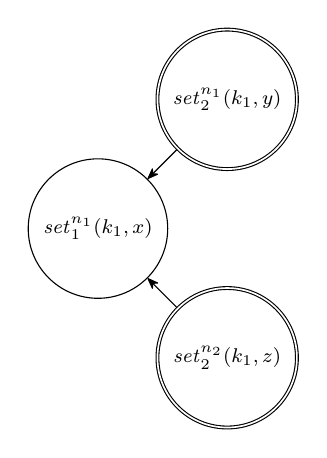
\begin{tikzpicture}[node distance=50pt]
		\small
		\def\dist{15pt}

		% nodes and edges
		\node[op] (k10) {\setop{1}{n_1}{k_1}{x}};

		\node[head,above right=\dist of k10] (k11) {\setop{2}{n_1}{k_1}{y}} edge [pred] (k10);
		\node[head,below right=\dist of k10] (k12) {\setop{2}{n_2}{k_1}{z}} edge [pred] (k10);

	\end{tikzpicture}
	\hskip8em
	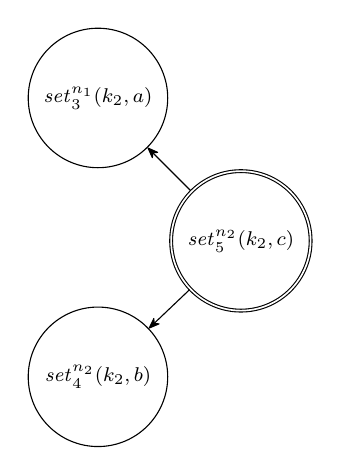
\begin{tikzpicture}[node distance=50pt]
		\small
		\def\dist{22pt}

		% nodes and edges
		\node[op] (k20) {\setop{3}{n_1}{k_2}{a}};
		\node[op,below=of k20] (k21) {\setop{4}{n_2}{k_2}{b}};

		\node[head,below right=\dist of k20] (k22) {\setop{5}{n_2}{k_2}{c}} edge [pred] (k20) edge [pred] (k21);

	\end{tikzpicture}
	\caption{
		The state from \autoref{tab:fact_tables} illustrated.
		The graph on the left depicts the operation history of the register with key \(k_1\)
		and the graph on the right of the register associated with key \(k_2\).
	}\label{fig:register_ops}
\end{figure*}

The causal history between the operations is illustrated on a logical level
in the graphs of \autoref{fig:register_ops}.
The edges denote the \code{pred} EDB and a node's
\setop{Counter}{NodeId}{Key}{Value} label denotes a base atom of the \code{set} EDB.
To obtain the state of the key value store, the following set must be computed:

\begin{align*}
	\var{mvrStore} = \{ (\var{Key}, \var{Value}) \mid & (\var{NodeId}, \var{Counter}, \var{Key}, \var{Value}) \in \var{set}                \\
	\land \text{ }                                    & \nexists (\var{FromNodeId}, \var{FromCounter}, \var{\_}, \var{\_}) \in \var{pred}: \\
	                                                  & \var{NodeId} = \var{FromNodeId} \land \var{Counter} = \var{FromCounter} \}
\end{align*}

With the state illustrated in \autoref{tab:fact_tables} and
\autoref{fig:register_ops}, the result
is \(\{ (k_1, y), (k_1, z), (k_2, c)\}\) because other assigned values
(\(x\) for \(k_1\); \(a, b\) for \(k_2\)) have been overwritten by later operations.
Formulating the query in Datalog is straightforward,
as it matches its mathematical counterpart quite well:

\begin{small}
	\begin{verbatim}
isPred(NodeId, Counter) :- pred(NodeId, Counter, ToNodeId, ToCounter)
mvrStore(Key, Value)    :- set(NodeId, Counter, Key, Value),
                           not isPred(NodeId, Counter)
\end{verbatim}
\end{small}

We may also use SQL to express this query. We show two variants.
The first one uses a \code{LEFT JOIN} and a \code{null} filter:

\begin{small}
	\begin{verbatim}
SELECT key, value
FROM set LEFT JOIN pred ON set.NodeId = pred.FromNodeId
                       AND set.Counter = pred.FromCounter
WHERE pred.FromNodeId IS NULL
\end{verbatim}
\end{small}

Alternatively, we can use a subquery and negated set inclusion,
to align the SQL query closer with the mathematical notation:

\begin{small}
	\begin{verbatim}
WITH isPred AS (SELECT FromNodeId, FromCounter FROM pred)
SELECT key, value FROM set WHERE (NodeId, Counter) NOT IN isPred
\end{verbatim}
\end{small}

While for this example the SQL queries are not too far off from the mathematical
notation, we think that Datalog is more elegant, offers better support for
composition, and excels at expressing recursion~\cite{abo2024convergence},
which is important for more complex CRDTs~\cite{kleppmann2018data}.
Especially, we want to avoid the cumbersome syntax around recursive
CTEs which remains unpopular even within the SQL
community~\cite{neumann2024critique, hirn2023fix, mcsherry2022recursion}.
Furthermore, there exists some interesting research about defining Datalog
over arbitrary semirings~\cite{abo2024convergence, khamis2022datalog},
which may lift Datalog's current restrictions around stratified negation and
stratified aggregation~\cite{green2013datalog}, and opens up new avenues for
Datalog's semantics.
We emphasize that recursion in SQL also suffers from requiring
monotonically growing sets for recursive queries~\cite{hirn2023fix},
just like recursion in Datalog.

\section{Connecting the Dots: CRDTs and Datalog}
\label{sec:crdts_datalog}

The literature defines two classes of CRDTs: state-based and operation-based
which both have different requirements for correctness.
Let \( S \) be the set of all possible states of a CRDT.
State-based CRDTs require a merge function \( \sqcup: S \times S \to S \)
which must be commutative, associative, and idempotent.
Operation-based CRDTs require that the operation functions \( op_i: S \to S \)
are commutative and applied exactly once.
Both models must adhere to these properties under the strong eventual consistency
model which demands three properties~\cite{shapiro2011comprehensive}:

\begin{enumerate}
	\item \textbf{Eventual Delivery}: All updates are eventually delivered to all replicas.
	\item \textbf{Termination}: All replicas eventually terminate.
	\item \textbf{Convergence}: All replicas that have delivered the same set of updates are in the same state.
\end{enumerate}

Verifying the correctness for a CRDT is a complex,
error-prone task~\cite{gomes2017verifying, kleppmann2022assessing},
and currently has to be done for each CRDT individually.
If, however, the set of operations on a CRDT \emph{is} the state,
the merge function can be defined as the set union,
for which the properties of commutativity, associativity, and idempotency hold.
The critical convergence property demanded by the strong eventual consistency
model is then also trivially satisfied because the state is by definition
the set of all (delivered) operations.
Moreover, applying any \emph{pure}\footnote{
	That is, the function is deterministic and side-effect-free.
}
function \( f: S \to T \) on the state does not impede the convergence property,
as the function is applied on all replicas in the same deterministic way.
\( T \) is an arbitrary set of all possible derived states \( f \) can map to.
This approach to CRDTs is known in the literature as
\emph{pure operation-based replicated data types}~\cite{baquero2017pure, stewen2024undo}
and used in practice in the Automerge CRDT~\cite{automerge}.

The pure function \( f \) can be expressed in a Datalog query.
As Datalog evaluation is deterministic, the convergence property is satisfied.
This gives application developers the power to define their own, custom CRDTs
without worrying about the complex aspect of convergence.
Furthermore, the query engine running the Datalog program is responsible
for finding an efficent algorithm to execute the query and application developers
can focus on the CRDT at a declarative level and get the implementation ``for free''.

A common pattern of collaboration is near-real-time collaboration on a shared
document and CRDTs can be used to power this form of collaboration.
In this scenario, updates are usually frequent but small and therefore it
may make sense to reuse the result of a previous query along with the input
delta in hope of saving computation time over recomputing the query from scratch
based on the whole input with every update.
Ideally, the computation time is only proportional to the size of the input
change but not to the whole input size anymore.
As older, causually overwritten updates to a CRDT are often not contributing
to the current state of the CRDT anymore, incremental view
maintenance (IVM)~\cite{mcsherry2013differential, budiu2022dbsp, budiu2024dbsp}
can turn out to be an essential aspect to make CRDTs expressed as
queries over relations feasable.

\section{System Overview and Theoretical Considerations}
\label{sec:system_overview}

We provide a system overview of the approach in \autoref{fig:system_overview}.
The \emph{database layer} incrementally updates the views \deltaO{},
as defined by the CRDT Datalog queries formulated on the \emph{application layer},
in response to updates from both the local \deltaI{local} and remote replicas
\deltaI{remote}.
In this model we assume that the application layer is responsible for forwarding
the updates to the database layer but the database layer could theoretically
also be responsible for that.
Moreover, \autoref{fig:system_overview} illustrates a peer to peer architecture
but, due to the lack of hierarchy, different network topologies are also possible,
e.g., a star network topology with a central server for more efficient update
propagation.
Yet, the issue of update propagation is not the focus of this research and
various approaches exist in the literature~\cite{auvolat2019merkle, sanjuan2020merkle}.
This also excludes the question of how to efficiently send just the minimum
set of missing updates to each replica.
We only make the basic assumption of some network topology and protocol
that ensures that each update will eventually be delivered to all replicas.

The DBSP paper~\cite{budiu2022dbsp} defines some theoretical foundation for IVM,
which is based on the algebraic structure of commutative groups
to model updates to multisets upon which relational algebra is relying on.
DBSP requires the time axis of the stream of updates to the inputs of the
queries it maintains to be totally ordered.
Coordination-free systems usually preclude total orders, at least the ones which
are final and not subject to change after the fact.
However, this is not an issue here as writes (in the sense of leightweight
transactions which may include individual updates to multiple relations)
can be ordered differently but totally on each replica in delivery order.
The use of CRDTs on the application layer can absorb the different orderings
of writes among replicas and still converge to the same state
if replicas have delivered the same set of writes.
Furthermore, the database layer must be capable of atomically updating all affected
relations of a write to safeguard the CRDT queries against reading inconsistent
state, i.e., queries read from a consistent snapshot of the database.
For instance, in the example of \autoref{sec:motivating_example} a logical update
to the key-value store touches both EDBs \code{set} and \code{pred}
simultaneously.
Hence, the database layer has to ensure that the two EDBs are updated atomically
such that reads either see both updates or none but not just one of them.

The CRDTs formulated in Datalog also rely on two algebraic structures.
The set of all operations of the CRDT \(S\) together with
the ``merge'' function defined as the set union (\(\cup\)) forms a semilattice
because it is associative, commutative, and idempotent.
The associativity and commutativity properties are key to absorbing
different write orderings.
Semilattices possess a link to order theory because their binary operation
induces a partial order between the elements of \(S\) through
\(s_1 \leq s_2 \Leftrightarrow s_1 \cup s_2 = s_2\).
Moreover, Datalog itself can be modeled as a semiring with
disjunction (\(\lor\)) and conjunction (\(\land\)) as the semiring's
binary operations, and in abstracting over these two concrete instances
of binary operations lies the potential to expand Datalog's expressiveness
towards new horizons~\cite{abo2024convergence}.

\begin{figure*}
	\centering

	\newcommand{\replica}{
		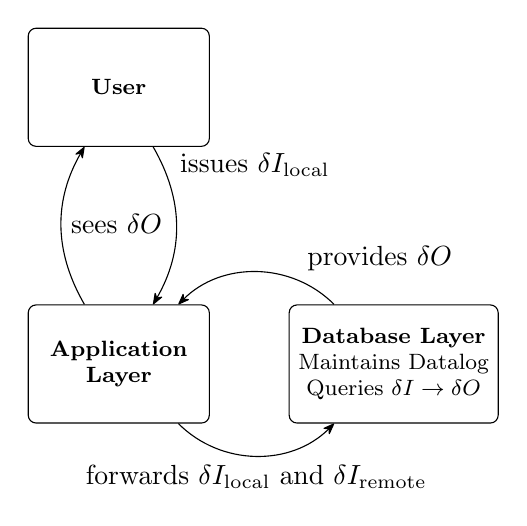
\begin{tikzpicture}
			\tikzset{
			layer/.style={
					rectangle, draw, minimum height=1.5cm, minimum width=2.3cm,
					rounded corners=1mm,
					font=\footnotesize, align=center,
				},
			rel/.style={
			->, >={Stealth[round]}, },
			}
			\node[layer] (app) {\textbf{Application}\\ \textbf{Layer}};
			\node[layer,right=of app] (db) {
				\textbf{Database Layer}\\
				Maintains Datalog\\
				Queries \(\delta I \to \delta O\)
			};
			\node[layer,above=2.0cm of app] (user) {\textbf{User}};

			\draw[rel] (user) to["issues \deltaI{local}", bend left, near start] (app);
			\draw[rel] (app) to["sees \deltaO", bend left,auto=right] (user);

			\draw[rel] (app) to["forwards \deltaI{local} and \deltaI{remote}", bend right=45, auto=right] (db);
			\draw[rel] (db) to["provides \deltaO", bend right=45, auto=right,near start] (app);
		\end{tikzpicture}
	}

	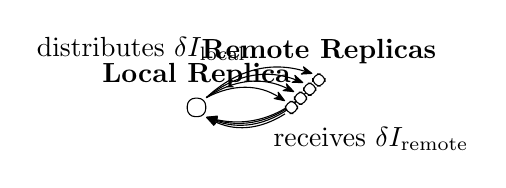
\begin{tikzpicture}
		\tikzset{
		replica/.style={rectangle, draw, rounded corners=1mm,fill=white},
		local_replica/.style={replica},
		remote_replica/.style={replica,scale=0.66},
		label/.style={font=\bfseries},
		rel/.style={
		->, >={Stealth[round]},bend left,},
		}

		\node[local_replica] (local) {\replica};
		\node[label] (local-label) [above=0pt of local] {Local Replica};

		\node[remote_replica] (remote3) [right=of local,yshift=+15pt,xshift=+15pt] {\replica};
		\node[remote_replica] (remote2) [right=of local,yshift=+10pt,xshift=+10pt] {\replica};
		\node[remote_replica] (remote1) [right=of local,yshift=+5pt,xshift=+5pt] {\replica};
		\node[remote_replica] (remote0) [right=of local] {\replica};
		\node[label] (remote-label) [above=0pt of remote3] {Remote Replicas};

		\begin{scope}[on background layer]
			\draw[rel] (local.north east) to[] (remote0.north west);
			\draw[rel] (local.north east) to[] (remote1.north west);
			\draw[rel] (local.north east) to[] (remote2.north west);
			\draw[rel] (local.north east) to["distributes \deltaI{local}"] (remote3.north west);

			\draw[rel] (remote0.south west) to[] (local.south east);
			\draw[rel] (remote1.south west) to[] (local.south east);
			\draw[rel] (remote2.south west) to[] (local.south east);
			\draw[rel] (remote3.south west) to["receives \deltaI{remote}"] (local.south east);
		\end{scope}

	\end{tikzpicture}

	\caption{
		An overview of the system architecture from the perspective of a local
		replica.
		\deltaI{local} and \deltaI{remote} refer to the input deltas to
		the EDBs from the local and remote replicas, respectively.
		\deltaO{} models the output delta of all Datalog queries and is based on
		the current state of the EDBs on the respective replica.
	}\label{fig:system_overview}
\end{figure*}

\section{Advanced Example: Respecting Causal Order}

Without the assumption of a causal broadcast,
the example from \autoref{sec:motivating_example} is not quite a proper MVR
but a register with not only the causal readiness but also the delivery
time at a node determining the current value(s) of the register.
To illustrate this issue, consider \autoref{fig:causal_issue} from the
perspective of replica \(n_2\).
We distinguish between a write's delivery time, denoted as \(t^d_i\),
and a write's causal order, denoted as \(t^c_i\).
The write's respective order along the two dimensions is given by the subscript
index \(i\).
Initially, replica \(n_2\) is in the familiar state from \autoref{fig:register_ops}.
Then, the two writes \(w_1\) and \(w_2\) from replica \(n_1\) are delivered to \(n_2\)
but in reverse order of their causal order
(\(w_1 < w_2\) according to \(t^c\) but \(w_1 > w_2\) according to \(t^d\)).
Without a causal broadcast, the query from \autoref{sec:motivating_example}
would return \(\{ (k_1, y_1), (k_1, z), (k_1, y_3)\} \) at time \(t^d_1\)
but the correct result respecting causal order
is \(\{ (k_1, y_1), (k_1, z) \}\), delivering the value \(y_3\) too early by
eagerly appling the update \(w_2\) without awaiting its causal dependency
\(w_1\) first.
If \(w_1\) is eventually delivered, the query ``jumps'' to the result
\( \{ (k_1, y_3) \} \) at time \(t^d_2\), skipping the intermediate state
that overwrites the conflicting values \(y_1\) and \(z\) with \(y_2\),
suggesting that the value \(y_3\) suddenly overwrote its previously reported
siblings \(y_1\) and \(z\).

To fix this issue, the query has to be adjusted.
The problem of causal delivery translates into a graph connectedness
problem: What nodes are reachable from the set of root nodes?
To answer that, we introduce three new Datalog rules:

\begin{small}
	\begin{verbatim}
isPred(NodeId, Counter) :- pred(NodeId, Counter, ToNodeId, ToCounter)
isSucc(NodeId, Counter) :- pred(FromNodeId, FromCounter, NodeId, Counter)
isRoot(NodeId, Counter) :- set(NodeId, Counter, Key, Value),
                           not isSucc(NodeId, Counter)
isCausallyReady(NodeId, Counter)
                        :- isRoot(NodeId, Counter)
isCausallyReady(NodeId, Counter)
                        :- isCausallyReady(FromNodeId, FromCounter),
                           pred(FromNodeId, FromCounter, NodeId, Counter)
mvrStore(Key, Value)    :- set(NodeId, Counter, Key, Value),
                           isCausallyReady(NodeId, Counter),
                           not isPred(NodeId, Counter)
\end{verbatim}
\end{small}

Translating this into SQL shows why we prefer Datalog for expressing recursion:

\begin{small}
	\begin{verbatim}
WITH isPred AS (SELECT FromNodeId, FromCounter FROM pred)
WITH isSucc AS (SELECT ToNodeId, ToCounter FROM pred)
WITH isRoot AS (SELECT NodeId, Counter FROM set
                WHERE (NodeId, Counter) NOT IN isSucc)
WITH RECURSIVE isCausallyReady AS (
    SELECT * FROM isRoot
    UNION [ALL]
    SELECT pred.ToNodeId, pred.ToCounter
    FROM pred, isCausallyReady
    WHERE pred.FromNodeId = isCausallyReady.NodeId
      AND pred.FromCounter = isCausallyReady.Counter
)

SELECT set.key, set.value
FROM set, isCausallyReady
WHERE set.NodeId = isCausallyReady.NodeId
  AND set.Counter = isCausallyReady.Counter
  AND (set.NodeId, set.Counter) NOT IN isPred
\end{verbatim}
\end{small}

While this issue can be ignored by simply assuming a causal broadcast
on the application layer,
we think that it undermines the approach's goals for two reasons.
First, a causal broadcast requires state to be kept on the application layer,
namely the buffer of writes which await the delivery of their causal dependencies.
Yet, this system is part of an effort to move state to the database
layer to render the application layer mostly stateless and potentially
have all state benefit from classical database guarantees like durability.
This extends the idea of functional reactive programming, as popularized
by React, to the whole application stack, including the database
layer, and allows the application to be considered a reactive, pure function
of some state captured in the EDBs~\cite{schiefer2022building}.
Second, it increases the complexity of the application layer by not allowing
it to treat the updates to the database as a black box beyond its forwarding
responsibilities.
Hence, we advocate to account for this issue on the query level at the expense
of an increased query complexity.

\begin{figure*}
	\centering
	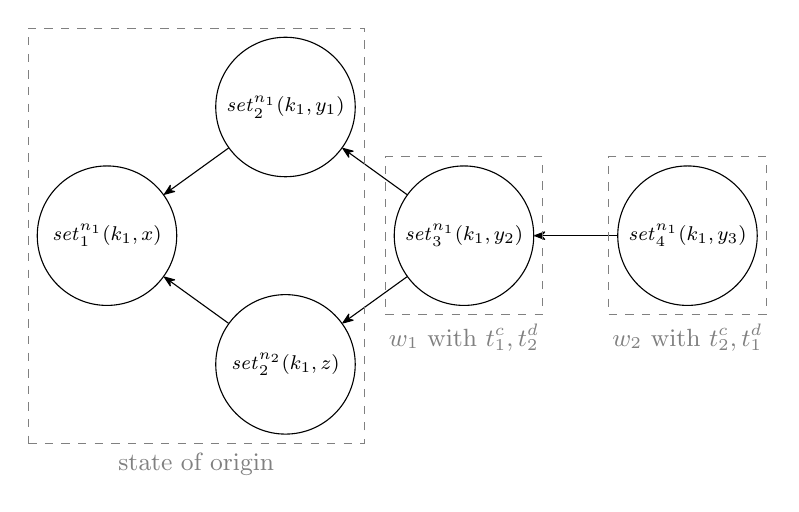
\begin{tikzpicture}[node distance=30pt]
		\small
		\def\dist{15pt}
		\def\shift{+20pt}

		\tikzset{
			tx/.style={draw=gray, dashed},
			tx_label/.style={text=gray, align=left, anchor=north}
		}

		% nodes and edges
		\node[op] (k10) {\setop{1}{n_1}{k_1}{x}};

		\node[op,above right=\dist of k10,xshift=\shift] (k11) {\setop{2}{n_1}{k_1}{y_1}}
		edge [pred] (k10);
		\node[op,below right=\dist of k10,xshift=\shift] (k12) {\setop{2}{n_2}{k_1}{z}}
		edge [pred] (k10);

		\node[op, below right=\dist of k11,xshift=\shift] (k13) {\setop{3}{n_1}{k_1}{y_2}}
		edge [pred] (k11) edge [pred] (k12);
		\node[op, right=of k13] (k14) {\setop{4}{n_1}{k_1}{y_3}}
		edge [pred] (k13);

		\node[tx,fit=(k10) (k11) (k12)] (tx0) {};
		\node[tx_label] at (tx0.south) {state of origin};
		\node[tx,fit=(k13)] (tx1) {};
		\node[tx_label] at (tx1.south) {\(w_1\) with \(t^c_1, t^d_2\)};
		\node[tx,fit=(k14)] (tx2) {};
		\node[tx_label] at (tx2.south) {\(w_2\) with \(t^c_2, t^d_1\)};

	\end{tikzpicture}
	\caption{
		Example of a causality issue with the naive queries from \autoref{sec:motivating_example}.
	}\label{fig:causal_issue}
\end{figure*}

\section{Contributions}
\label{sec:problem_stmnt}

The goals of this research are twofold:
First, we deal with the question if Datalog is expressive and ergonomic enough
to express common CRDTs.
To answer that question, we implement common CRDT types in Datalog, e.g.,
a list/sequence CRDT, a map CRDT, as well as a set CRDT,
and evaluate our experience.
Queries often involve negation (see \autoref{sec:motivating_example})
and because core Datalog does not support negation, the question arises if
the most commonly used Datalog extension for negation,
stratified negation~\cite{green2013datalog}, is expressive enough.

Second, we turn to the question of the practical performance of this approach.
We want to test some CRDT workloads against our CRDT Datalog implementations and
evaluate the performance.
To do so, we (1) may have to define common CRDT workloads for benchmarking
(unfortunately, there is no standard like TPCH established yet\footnote{
	There are some benchmarks for text editing:
	\url{https://github.com/dmonad/crdt-benchmarks} and
	\url{https://github.com/josephg/editing-traces}.
}), and we (2) either utilize some existing Datalog engines and test them
with and without incremental view maintenance or may have to deal with
prototyping our own, as support for incremental view maintenance is variable
among Datalog engines
(see \autoref{tab:datalog-engines} for a non-exhaustive overview).

Ideally, this different approach to CRDTs would move them closer to the power,
guarantees and flexibility of database systems.
The higher abstraction of a query language better supports the decoupling from
logical and physical data representations than object-oriented APIs,
and a higher abstraction allows for optimizations without breaking changes,
something relational databases have benefitted from over the years and has
arguably contributed towards their widespread adoption.
Furthermore, the read finality issue of CRDTs under non-monotone queries
may be better addressed with the support of a query language~\cite{laddad2022keep}.
On the other hand, database systems can be introduced to coordination-free
environments.
In exchange for some guarantees which cannot be upheld
like for instance uniqueness constraints,
coordination-free database systems can deliver ultimate availability
to their clients:
As long as the client, which \emph{is} a replica of the distributed database,
is alive, the system is available.
This property can be useful in contexts where a network partition would be
prohibitively expensive to tolerate such as manufacturing processes,
which cannot afford to stop an entire production facility just because
some server is not available.

\begin{table*}[]
	\center
	\small
	\begin{tabular}{@{}lp{3.4cm}lp{1.2cm}p{0.7cm}l@{}}
		\toprule
		Engine                                                                      & Datalog Variant                          & IVM & Language  & Open Source & Active \\
		\midrule
		\href{https://github.com/souffle-lang/souffle}{Souffle}                     & With stratified negation                 & No  & C++       & Yes         & Yes    \\
		\href{https://github.com/rust-lang/datafrog}{Datafrog}                      & Vanilla                                  & No  & Rust      & Yes         & No     \\
		\href{https://github.com/vmware/differential-datalog}{Differential Datalog} & ?                                        & Yes & Rust/Java & Yes         & No     \\
		\href{https://github.com/s-arash/ascent/}{Ascent}                           & With stratified negation and aggregation & No  & Rust      & Yes         & Yes    \\
		\href{https://github.com/ekzhang/crepe}{Crepe}                              & With stratified negation                 & No  & Rust      & Yes         & No     \\
		\href{https://github.com/knowsys/nemo}{Nemo}                                & Based on RDF instead of relations        & ?   & Rust      & Yes         & Yes    \\
		\href{https://www.datomic.com}{Datomic}                                     & Custom (and appears to use RDF)          & ?   & Clojure   & No          & Yes    \\
		\href{https://github.com/tonsky/datascript}{Datascript}                     & Appears to mimic Datomic                 & ?   & Clojure   & Yes         & Yes    \\
		\href{https://github.com/comnik/declarative-dataflow}{Declarative Dataflow} & ?                                        & Yes & Rust      & Yes         & No     \\
		\bottomrule
	\end{tabular}
	\caption{Overview of some Datalog Engines}
	\label{tab:datalog-engines}
\end{table*}

\pagebreak{}
\printbibliography{}

\end{document}
